\chapter{Model of the system}
In order to calculate the participation ratio of the different lossy layers in an arbitrary structure, it is simulated using 3D EM simulation software called Computer Simulation Technology Studio Suite (CST). Certain assumptions and simplifications are made to allow for simulation within CST. These are discussed below. A step-by-step guide for setting up a simulation in CST can be found in appendix \ref{appendix:CST_procedure}.
%reduce simulation times and \ldots. 

\section{Materials and dimensions}
Certain choices of materials and dimensions are valid for all qubit designs in this project. They are listed in table \ref{table:standard_parameters} below.

\begin{table}
	\begin{center}
		\begin{tabular}{ | l || c | c | c |}
			\hline
			 & Material & Thickness & Permeability \\ \hline
			Pads & PEC & 10 um & 1 \\
			Substrate & Silicon & 520 um & 1 \\
			Ground & PEC & - & 1 \\
			MA & NiO & \textasciitilde 3 nm & 1 \\
			MS &  & \textasciitilde 3 nm & 1 \\
			SA & SiO & \textasciitilde 3 nm & 1 \\
			\hline
		\end{tabular}
	\end{center}
	\caption{Parameters that are valid for all qubit designs used in this research}
	\label{table:standard_parameters}
\end{table}


\section{Josephson junction}
During simulation in CST, the Josephson junction is replaced by an inductor. By tuning the inductance together with the capacitance of the structure a specific resonance frequency can be reached (see formula \eqref{}). 


\section{Lossy layers}
The relatively small thickness of the layers suggests that the impact they have on the Electric field is small \todo{SOURCE?}. During simulation their impact is neglected and the layers are therefore omitted. The exclusion of thin lossy layers prevents the necessity for mesh elements with sub-nano meter size. This significantly reduces the number of mesh elements and in turn the computation time of the simulation. A simple representation of the structure can be seen in figure~\ref{fig:model}.
\begin{figure}
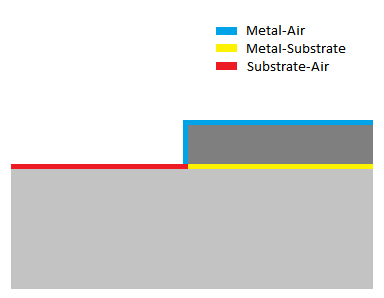
\includegraphics[scale=.8]{Figures/model}
\caption{Simplification of the system including three lossy layers. The substrate and metal are depicted in light and dark grey respectively}
\label{fig:model}
\end{figure}

\section{Meshing}
To reduce simulation times the initial mesh is of critical importance. After each mesh refinement the fields are simulated anew. While CST is able to select regions of importance in the system where it should further refine the mesh, it can only do so after having simulated the fields. When establishing the initial mesh the importance of different regions of the system must be taken into account. Two \todo{two?} important steps taken to improve the initial mesh during this project are described below.   


\subsection{Ground}
To reduce the number of mesh elements, the ground pad is replaced by a sheet of PEC with zero thickness. Considering the field in the ground region is small compared to the field at the edges of the pads its contribution to the participation ratio is also small. Investing more computation time on the ground plane region by increasing the density of mesh elements there, would therefore also have limited impact on the participation ratio.
\subsection{Pads}
The pads being the source of the electric field, it is to be expected that the intensity will be greatest in this region. Furthermore, electric field lines tend to have a higher density at the edges of a metal \todo{Source or reference to Theory}. Considering this, the intensity of the electric field in the entire system is expected to be greatest around the edges of the metal pads. The initial mesh should reflect this by being very fine in these regions. In order to achieve this the edges of the metal pads are rounded as in figure \ref{fig:blending} of the appendix \todo{Print figure here as well, including resulting mesh?}.The steps taken to achieve this in CST can be found in appendix \ref{appendix:CST_procedure}. 